\section{Limity równoległych zapytań dla zbioru FWB\_0}

\begin{figure}[!hb]
	\centering 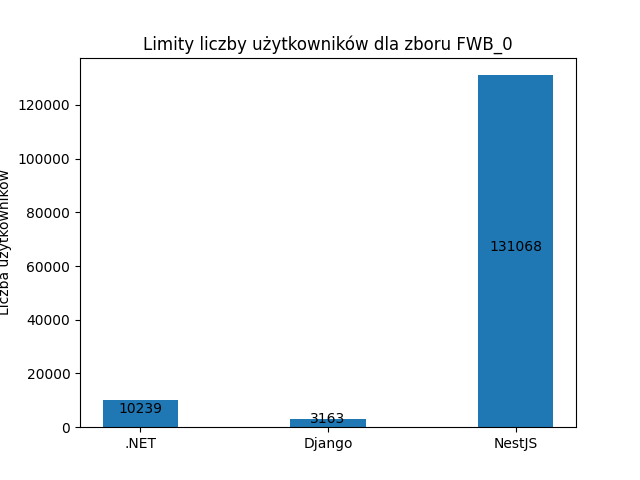
\includegraphics[width=1\linewidth]{rysunki/Limity_liczby_uzytkownikow_dla_zboru_FWB_0.png}
	\caption{Limit liczby użytkowników przy zwracaniu zbioru FWB\_0}
	\label{rys:limit_vus_fwb_0}
\end{figure}

Wyniki badania limitu równoległych zapytań zostały zaprezentowane na rysunku \ref{rys:limit_vus_fwb_0}.

Zestawienie zostało zdominowane przez NestJS, które uzyskało wynik na poziomie ponad 131 tysięcy użytkowników.
Kolejny na podium uplasował się .NET z 13-krotnie niższym limitem na poziomie 10 tysięcy.
3-krotnie niższy od .NET limit przypadł Django z wynikiem na poziomie 3 tysięcy.
